\section{Durchführung}
%
\begin{figure}[!htbp]
\centering
\resizebox{\textwidth}{!}{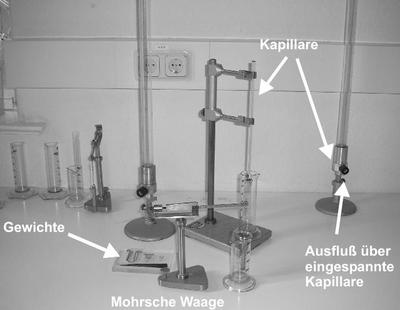
\includegraphics{versuchsaufbau.jpg}}
\caption{Versuchsaufbau \cite{LP:Online}}
\label{img:aufbau}
\end{figure}
%
Vor dem Versuch werden die Kapillaren gründlich mit destilliertem Wasser und Lösungsmittel gereinigt und sorgfältig getrocknet. Mit einem Messmikroskop werden die Radien der Kapillaren mehrfach gemessen.
%
\subsection{Kapillarität}
Es werden drei Flüssigkeiten untersucht: Destilliertes Wasser, Methanol und Ethylenglykol. Die Kapillaren werden in die zu untersuchende Flüssigkeit getaucht und bis an die Oberfläche herausgezogen. Der entstehende Höhenunterschied $h_{\text{kap}}$ wird für jede Kombination aus Kapillare und Flüssigkeit drei mal bestimmt. Dabei ist darauf zu achten, dass die Kapillare vor der Messung trocken sind und vor dem Wechsel der Flüssigkeit nochmals gereinigt werden.\\
Mit einer Mohrschen Waage werden die Dichten $\rho$ der Flüssigkeiten bestimmt. Der Probekörper sollte vor jeder Messung trocken und sauber sein und ganz in die Flüssigkeit eintauchen.
%
\subsection{Innere Reibung}
%
\begin{figure}[!htbp]
\centering
\resizebox{0.5\textwidth}{!}{\input{skizze_teil2.pdf_tex}}
\caption{Skizze zum zweiten Versuchsteil \cite{LP:Online}}
\label{img:skizze_teil2}
\end{figure}
%
Zunächst werden der Durchmesser des Glasgefäßes, die Länge der Kapillaren und die Temperatur des destillierten Wassers gemessen. Abbildung \ref{img:skizze_teil2} zeigt den eigentlichen Versuchsaufbau.\\
Die drei Kapillaren werden nacheinander in die Öffnung des Glasgefäßes gesteckt. Für jede Kapillare wird die Ausflusszeit von destilliertem Wasser zwischen den Strichmarken 50 und 45 mit einer Stoppuhr gemessen.\\
Für die kleinste Kapillare wird die Zeit in Abhängigkeit von der Höhe der Wassersäule über einen längeren Zeitraum gemessen.